\documentclass[preprint,12pt]{elsarticle}

\usepackage{amsmath,amssymb}
\usepackage{booktabs}
\usepackage{multirow}
\usepackage{graphicx}
\usepackage{adjustbox}
\usepackage{subcaption}
\usepackage{siunitx}
\usepackage{enumitem}
\usepackage{xcolor}
\usepackage{hyperref}
\usepackage{url}
\usepackage{float}
\usepackage[section]{placeins}

\journal{Computer Methods and Programs in Biomedicine}
\graphicspath{{figures/}{./}}
\hypersetup{
    hidelinks,
    pdftitle={A Reproducible ROI-Robust Evaluation and Mobile Distillation Framework for Ultrasound Lesion Classification},
    pdfauthor={Zihan Li and Cong Yang}
}
\pdfstringdefDisableCommands{%
    \def\corref#1{}%
}
\setlength{\emergencystretch}{2em}

\begin{document}

\begin{frontmatter}

\title{A Reproducible ROI-Robust Evaluation and Mobile Distillation Framework for Ultrasound Lesion Classification}

\author[inst1]{Zihan Li}
\author[inst1]{Cong Yang\corref{cor1}}
\ead{cong.yang@suda.edu.cn}
\cortext[cor1]{Corresponding author.}

\affiliation[inst1]{organization={School of Future Science and Engineering, Soochow University},
            city={Suzhou},
            postcode={215222},
            state={Jiangsu},
            country={China}}

\begin{abstract}
\textbf{Background and Objective:}
Ultrasound lesion classification is sensitive to lesion localization, domain-specific image appearance, and deployment constraints. Annotation-derived region-of-interest (ROI) crops often give strong classifier results, but they can overstate practical feasibility if localization error, model-selection provenance, and real-device latency are not evaluated.
\textbf{Methods:}
We present a reproducible ROI-based evaluation and mobile-distillation framework across thyroid, breast, and liver public datasets. The framework uses a TransXNet-family model as a high-capacity teacher and design-space probe, evaluates coordinate-aware refinement, multi-scale dynamic dense reuse, and differential attention under a validation-fixed protocol, and then distills efficient students for Android deployment. We separate oracle ROI, synthetic box perturbation, detector-derived ROI, full-image controls, dataset-specific training, joint multi-organ training, and leave-one-domain-out transfer.
\textbf{Results:}
On TN5000, full-factorial ablation shows that dynamic dense reuse plus differential attention is the most reliable TransXNet-family configuration (ensemble AUC 0.9618, balanced accuracy 0.9028), while coordinate-aware refinement is dataset-dependent rather than uniformly beneficial. The best robustness variant degrades gradually from GT ROIs to 5\%, 10\%, 20\% perturbed ROIs and detector boxes, with AUCs of 0.9623, 0.9594, 0.9556, 0.9463, and 0.9497, respectively. On Xiaomi and Samsung Android devices, an EfficientFormer-L1 student distilled from the teacher reaches 0.9634 exported TN5000 AUC with 32.7/56.0 ms hot end-to-end latency, compared with 0.9433 AUC and 130.6/168.4 ms for the exported TransXNet-family teacher artifact under the same paper-log analysis-label snapshot. Joint multi-organ EfficientFormer training remains feasible, but leave-one-domain-out transfer is weak. A BUSI duplicate audit further shows why the breast results should be interpreted as public-benchmark evidence rather than a cleaned clinical estimate.
\textbf{Conclusions:}
The evidence supports ROI-robust ultrasound classification and a practical teacher-student mobile path, while identifying clear limits for zero-shot cross-organ transfer and clinical deployment readiness.
\end{abstract}

\begin{keyword}
Ultrasound image classification \sep Region of interest \sep Localization robustness \sep Reproducible evaluation \sep Knowledge distillation \sep Mobile inference
\end{keyword}

\end{frontmatter}

\section{Introduction}
\label{sec:introduction}

Ultrasound is widely used for screening, follow-up, and diagnostic support because it is inexpensive, radiation-free, portable, and suitable for repeated acquisition. These advantages also create a difficult computer-aided diagnosis setting. Speckle noise, weak lesion boundaries, low contrast, operator dependency, and device-dependent appearance shifts can obscure benign--malignant cues. Deep learning has improved ultrasound classification, but practical lesion classifiers still face three linked problems: they often depend on annotation-derived ROI crops, they can be tuned to one dataset protocol, and their reported efficiency may not translate to real-device latency.

This paper targets that gap from a computing-methods perspective. Rather than presenting a new universal medical vision backbone, we study an ROI-robust ultrasound lesion-classification framework that connects controlled ROI classification, localization-error analysis, model-selection provenance, and Android feasibility. TN5000 thyroid nodules are used as the primary benchmark~\cite{Zhang_2025}, while BUSI breast lesions~\cite{Al_Dhabyani_2020} and the Annotated Ultrasound Liver (AUL) dataset~\cite{aul_dataset} provide additional public in-domain benchmarks from different organs. These datasets differ in anatomy, acquisition appearance, annotation protocol, and class prevalence, so they should not be treated as automatic evidence of zero-shot cross-organ generalization.

The core methodological question is how to organize a compact but accurate ROI classifier when lesion crops may be imperfect. We use a TransXNet-family teacher~\cite{transxnet} as a high-capacity ROI model and study three adaptations: coordinate-aware feature refinement inspired by coordinate attention~\cite{hou2021coordinate}, multi-scale dynamic dense reuse, and differential attention adapted from the Differential Transformer formulation~\cite{ye2024differential}. We then decouple the accuracy-oriented teacher analysis from deployment by distilling EfficientFormer-L1 students~\cite{li2022efficientformer} and measuring them on a real Android device.

The contributions are:
\begin{itemize}[leftmargin=1.5em]
    \item We provide a validation-fixed, reproducible ROI ultrasound lesion-classification protocol with explicit label-snapshot provenance and case-level prediction artifacts.
    \item We analyze a modular TransXNet-family teacher with full-factorial MCA/MUDD/DA ablation, showing that MUDD and differential attention are the most reliable TN5000 contributors, while MCA is dataset-dependent.
    \item We quantify localization robustness using GT boxes, synthetic box perturbations, detector-derived boxes, and full-image controls.
    \item We introduce a teacher-student deployment path in which Efficient\-Former-L1 students preserve high TN5000 discrimination while reducing real-device Android latency.
    \item We distinguish multi-organ joint training from leave-one-domain-out transfer, showing that the former is feasible but true zero-shot cross-organ generalization remains limited.
\end{itemize}
\FloatBarrier

\section{Related work}
\label{sec:related_work}

Deep learning is now central to medical image analysis~\cite{litjens2017survey}, but ultrasound remains difficult because acquisition conditions, speckle, boundary ambiguity, and annotation quality vary substantially across datasets. Clinical reporting systems such as ACR TI-RADS for thyroid ultrasound~\cite{tessler2017tirads} and BI-RADS for breast imaging~\cite{acr_birads} also emphasize morphology, margin, and contextual appearance rather than isolated texture alone. Earlier breast-ultrasound classification work already showed that ROI definition and feature design strongly affect benign--malignant discrimination~\cite{G_mez_Flores_2015}. More recent ultrasound studies have explored multi-view learning for tumor classification~\cite{Luo_2023}, segmentation-oriented architectures~\cite{Chen_2023}, lightweight real-time models~\cite{Wang_2024,Ren_2025}, dataset curation for BUSI~\cite{aumente2025curatedbusi}, and ultrasound foundation-model pretraining~\cite{meyer2024ultrasam}. These studies motivate the present focus on the interface between lesion localization, ROI classification, data quality, and computational efficiency rather than on accuracy alone.

Efficient vision backbones provide another relevant line of work. CNNs and modern hybrid models such as ConvNeXt, Swin Transformer, RepViT, EfficientFormer, and TransXNet show different trade-offs among parameters, MACs, GPU latency, and mobile latency~\cite{liu2021swin,liu2022convnext,repvit,li2022efficientformer,transxnet}. In medical ultrasound, however, parameter count alone is not a sufficient deployment claim. Preprocessing, TTA, model export, runtime delegate choice, and device-specific kernels can dominate practical latency. This is why our evaluation separates the high-capacity TransXNet-family teacher from the distilled EfficientFormer student.

Finally, robustness and reporting transparency are important for clinical AI. Calibration errors can make probability outputs unreliable even when AUC is high~\cite{guo2017calibration}, and imperfect medical annotations or localization errors can change downstream performance~\cite{tajbakhsh2020embracing}. We therefore report validation-fixed selection, case-level confidence intervals, detector-derived ROI experiments, and leave-one-domain-out probes. These are not add-on diagnostics; they define the claim boundary of the method.

\section{Methods}
\label{sec:methods}

\subsection{Problem setting and ROI construction}

Given an ultrasound image and a lesion region, the classifier predicts a binary label $y \in \{0,1\}$, where $0$ denotes benign and $1$ denotes malignant. The model produces logits $z=f_\theta(x)$ and a malignant posterior
\begin{equation}
    p(y=1\mid x)=\frac{\exp(z_1)}{\exp(z_0)+\exp(z_1)}.
\end{equation}
The main protocol constructs expanded lesion-centered ROI crops from annotation boxes, as summarized in Fig.~\ref{fig:roi_preprocessing}. The box is expanded around the lesion center, clipped to the image boundary, resized to the model input size, and normalized. This oracle-ROI setting isolates classifier behavior and represents a controlled upper-bound input. We additionally evaluate detector-derived boxes and full-image inputs to estimate practical loss when annotation boxes are unavailable.

\begin{figure}[H]
    \centering
    
\includegraphics[width=0.82\textwidth]{fig_roi_preprocessing.png}
    \caption{ROI input construction. The lesion annotation defines an initial box, which is expanded while preserving aspect ratio and then resized to the classifier input size.}
    \label{fig:roi_preprocessing}
\end{figure}

\subsection{TransXNet-family teacher}

The teacher is a TransXNet-family hierarchical local--global backbone. It follows a four-stage configuration with stage depths $[4,4,15,4]$, embedding dimensions $[48,96,224,448]$, head numbers $[1,2,4,8]$, and spatial-reduction ratios $[8,4,2,1]$. For compatibility with the original implementation and the saved experimental checkpoints, the backbone is configured with a 1000-D trainable task projection before the binary head. This vector is not interpreted as ImageNet class probabilities; it is fine-tuned end-to-end as an intermediate representation and then passed to a 1000--512--2 MLP head.

\begin{figure}[H]
    \centering
    
\includegraphics[width=0.93\textwidth]{fig_architecture_crop.pdf}
    \caption{TransXNet-family ROI teacher used for high-capacity ultrasound lesion classification. The teacher supports modular analysis of coordinate-aware refinement, multi-scale dynamic dense reuse, and differential attention before distillation into an efficient mobile student.}
    \label{fig:architecture}
\end{figure}

We study three modular adaptations. Multi-scale coordinate attention (MCA) is a coordinate-aware refinement option for spatially selective feature recalibration. Multiway dynamic dense connection (MUDD) is inserted before the token-mixer residual branch in blocks from stage 2 onward. Within each stage, it stores at most four previous block outputs and resets the cache at stage boundaries. For a current feature map $x_l\in\mathbb{R}^{B\times C\times H\times W}$, MUDD first splits channels into $P=4$ equal paths $x_{l,p}$. A lightweight global gate produces a path-mixing matrix
\begin{equation}
    W_l=\mathrm{softmax}\left(
    \mathrm{Conv}_{1\times1}\left(
    \phi(\mathrm{Conv}_{1\times1}(\mathrm{GAP}(x_l)))
    \right)\right)\in\mathbb{R}^{B\times P\times P},
\end{equation}
where $\phi$ is GELU. Each path is transformed by a depthwise $3\times3$ convolution and a pointwise $1\times1$ convolution, then receives spatially aligned same-path features from previous blocks:
\begin{equation}
    \tilde{x}_{l,p}=T_p(x_{l,p})+
    \sum_{j<l} W_l[:,p,j\bmod P]\,
    \mathrm{Resize}(x_{j,p};H,W).
\end{equation}
The path outputs are concatenated to recover $C$ channels and are then processed by the original TransXNet block. Thus MUDD is a dynamic feature-reuse connection, not a separate classifier head. Differential attention computes two attention maps and subtracts the second from the first:
\begin{equation}
    A_{\mathrm{diff}} =
    \mathrm{softmax}(Q_1K_1^\top/\sqrt{d})
    - \lambda\mathrm{softmax}(Q_2K_2^\top/\sqrt{d}),
\end{equation}
where $\lambda$ is learned. In this ROI-ultrasound setting, the module is interpreted as a way to suppress common background or speckle-like responses while sharpening lesion-related relational contrast. We do not claim these modules as new independent primitives; the contribution is their controlled reorganization and evaluation for ROI-robust ultrasound classification.

\subsection{Efficient mobile student}

The TransXNet-family teacher is parameter/MAC-efficient relative to several large baselines, but it is not optimized for real-device latency. We therefore train EfficientFormer-L1 students with teacher guidance. This separates two roles: the TransXNet-family model provides an accuracy-oriented teacher and design analysis, whereas the EfficientFormer student is the mobile candidate. For student training, teacher logits $z_t$ are generated from the validation-selected TransXNet-family teacher under the same TN5000 ROI preprocessing. The student logits $z_s$ are optimized with a standard supervised and distillation objective,
\begin{equation}
    \mathcal{L} =
    (1-\alpha)\mathcal{L}_{\mathrm{CE}}(y,\sigma(z_s))
    + \alpha \tau^2
    \mathrm{KL}\left(\sigma(z_t/\tau)\,\|\,\sigma(z_s/\tau)\right),
\end{equation}
where $\tau$ is the distillation temperature and $\alpha$ controls the supervised--teacher trade-off. In the reported TN5000 mobile runs, $\alpha=0.45$ and $\tau=3.0$. Students are trained for up to 70 epochs with early stopping patience 12, 30\% expanded annotation-derived ROI crops, 224-pixel EfficientFormer input, backbone/head learning rates of $5\times10^{-5}$ and $1.5\times10^{-4}$, weight decay $10^{-4}$, dropout 0.3, EMA, horizontal-flip TTA, temperature scaling, and top-3 checkpoint averaging. The EfficientFormer-L1+ECA variant adds a lightweight efficient-channel-attention refinement to the student feature stream before the binary head. Noisy or detector-derived ROIs are used for robustness evaluation, not for retuning the KD loss. Android deployment uses ONNX Runtime and the same TN5000 ROI preprocessing, calibration temperature, and decision-threshold logic used by the validation-selected pipeline.

\section{Datasets and experimental protocol}
\label{sec:protocol}

\subsection{Datasets}

Table~\ref{tab:datasets} summarizes the public datasets and split protocols. TN5000 uses the official train/validation/test split. BUSI and AUL use a fixed held-out test set and five training folds on the remaining trainval set; their mean and standard deviation therefore reflect training-fold variation evaluated on the same fixed test set, not an outer five-fold cross-validation estimate. BUSI is kept in its public benchmark form for comparability, but we additionally audit duplicate and near-duplicate candidates because prior work has reported BUSI curation issues~\cite{aumente2025curatedbusi}. The audit is reported in the supplementary material and is not used to silently change the main benchmark denominator.

\begin{table}[!htbp]
    \centering
    \small
    \caption{Datasets and protocol. Dataset-statistics counts follow the descriptive counts in the source datasets. New robustness and mobile analyses use a frozen file-level analysis-label snapshot associated with the final reported runs; this snapshot is reported separately for provenance and does not overwrite the descriptive dataset counts.}
    \label{tab:datasets}
    \begin{adjustbox}{max width=\columnwidth}
    \begin{tabular}{llllll}
        \toprule
        Dataset & Organ & Images & Dataset B/M & Analysis B/M & Split protocol \\
        \midrule
        TN5000 & Thyroid & 5000 & 1426/3574 & 1435/3565 & Official 3500/500/1000 \\
        BUSI & Breast & 647 & 437/210 & 435/212 & Fixed test 129; five trainval folds \\
        AUL & Liver & 635 & 200/435 & 183/452 & Fixed test 127; five trainval folds \\
        \bottomrule
    \end{tabular}
    \end{adjustbox}
\end{table}

\subsection{Training, selection, and reporting}

Models are trained with the same ROI construction, label mapping, metric computation, validation-derived threshold search, temperature-scaling procedure~\cite{guo2017calibration}, and test-time augmentation convention unless an exception is stated. Timm baselines use ImageNet-pretrained initialization where available and replace their classification heads with binary heads; custom TransXNet-family models use the same local training protocol and the 1000-D task-projection head described above. Architecture choices, calibration temperatures, and operating thresholds are selected on validation predictions. Test predictions are generated after each configuration is fixed.

The detector-derived ROI condition uses diagnosis-agnostic one-class YOLO11n lesion detectors trained only to localize lesion boxes. TN5000 detectors are trained on the official train split for three seeds, with validation on the official validation split and final localization/classification evaluation on the official test split. BUSI and AUL use one detector per training fold and evaluate detector boxes on the fixed held-out test set. Detector training uses 80 epochs, 640-pixel detector input, the best validation checkpoint, confidence threshold 0.001 at inference, IoU/NMS threshold 0.7 for the TN5000 pipeline, and the highest-confidence predicted box. If no box is returned, the auto-ROI evaluator records a no-detection case and falls back to the full image for the downstream crop. Detector weights are used only as an auxiliary front end; they are not presented as a detection-method contribution.

The main metrics are AUC, balanced accuracy (BalAcc), macro F1, accuracy, sensitivity, specificity, PPV, NPV, calibration error, and Brier score. For new robustness, mobile, and cross-protocol analyses, we use a frozen file-level analysis-label snapshot associated with the final reported runs and report confidence intervals by bootstrap resampling over test cases. This snapshot is kept separate from the descriptive dataset-statistics counts in Table~\ref{tab:datasets}. Because BUSI/AUL reuse a fixed held-out test set across five training folds and TN5000 repeated runs use the same official test set, the seed/fold standard deviations in benchmark tables quantify training-run variability on a fixed test population rather than independent outer-fold uncertainty. Strong ImageNet initialization, EMA, checkpoint averaging, and TTA can further reduce repeated-run AUC variance; case-level confidence intervals are therefore reported separately. The release package is organized around manifest files rather than aggregate counts: each case record contains the relative image path, original label, analysis label, split or fold, lesion box coordinates where available, exclusion flag, and the manifest hash used by the corresponding result table. Per-case prediction CSV files are linked to the same identifiers so that table metrics can be regenerated from case-level outputs.

\subsection{Compared protocols}

The experiments are grouped into four evidence blocks. First, full-factorial TN5000 ablation isolates MCA, MUDD, and differential attention. Second, ROI robustness evaluates GT boxes, synthetic box noise, detector boxes, and full images. Third, the mobile study compares the TransXNet-family teacher with EfficientFormer students and mobile baselines on an Android device. Fourth, the multi-organ study compares single-domain training, joint multi-organ training, and leave-one-domain-out (LODO) transfer. This structure is designed to prevent three common interpretation errors: treating multi-dataset in-domain testing as zero-shot generalization, treating parameter efficiency as mobile speed, and treating oracle ROI classification as a complete clinical workflow. Table~\ref{tab:model_roles} defines the names used across these blocks.

\begin{table}[!htbp]
    \centering
    \small
    \caption{Roles of the reported model configurations. The paper reports a teacher design space and a distilled mobile student rather than a single model that is optimal for every protocol.}
    \label{tab:model_roles}
    \begin{adjustbox}{max width=\columnwidth}
    \begin{tabular}{llll}
        \toprule
        Name & Structure & Primary role & Main evidence \\
        \midrule
        UL-TransXNet / GGG-MCA & MCA+MUDD+DA teacher & Dataset-specific benchmark & Tables~\ref{tab:main_benchmark}--\ref{tab:original_transxnet_delta} \\
        MUDD+DA-noMCA & MUDD+DA teacher & Robustness teacher & Tables~\ref{tab:factorial}--\ref{tab:roi_robustness} \\
        EfficientFormer-L1+KD & Distilled student & Mobile candidate & Table~\ref{tab:mobile} \\
        EfficientFormer-L1+ECA+KD & Distilled ECA student & Mobile/joint-training candidate & Tables~\ref{tab:mobile} and~\ref{tab:cross_organ} \\
        \bottomrule
    \end{tabular}
    \end{adjustbox}
\end{table}

\begin{figure}[H]
    \centering
    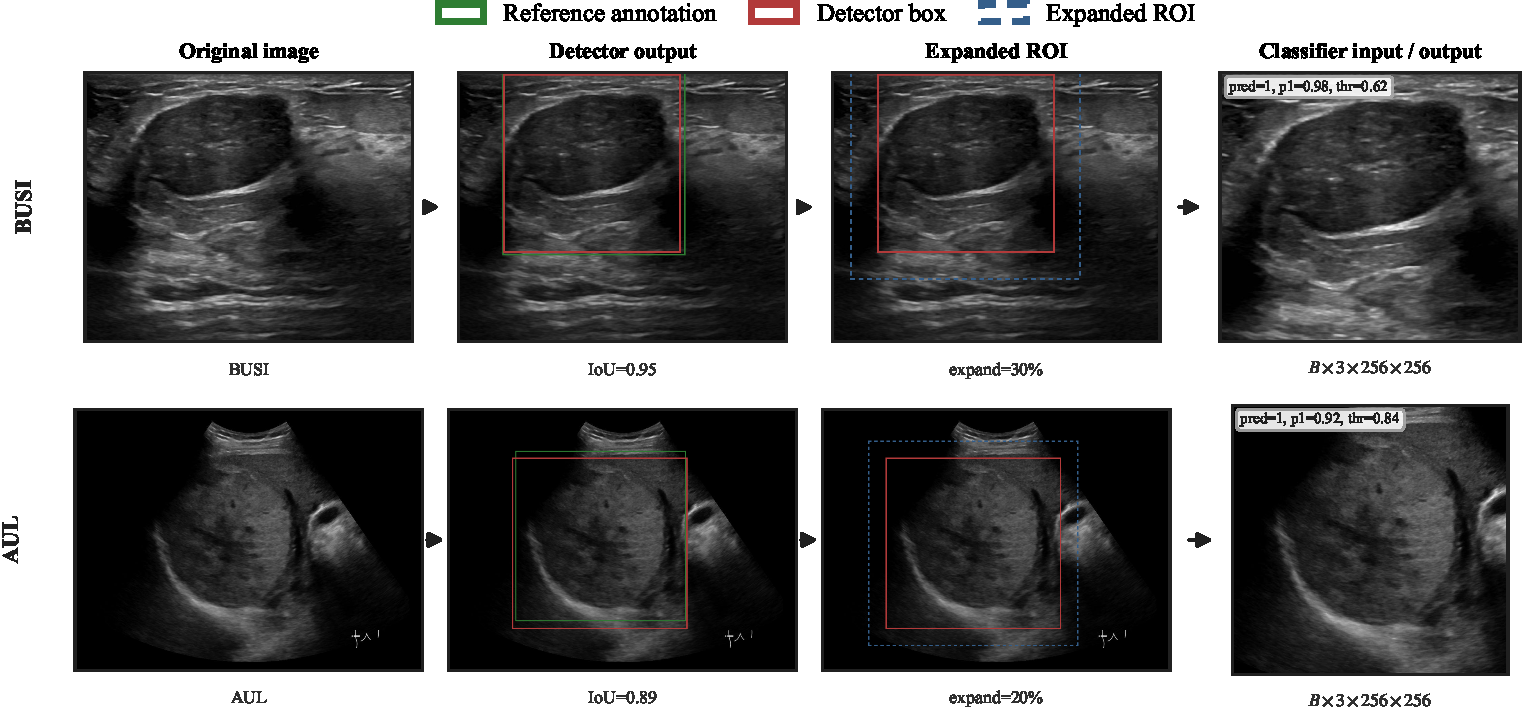
\includegraphics[width=0.95\textwidth]{fig_auto_roi_workflow_crop.pdf}
    \caption{Automatic ROI workflow used to connect the controlled oracle-ROI classifier to a detector-classifier inference setting. Green boxes indicate reference annotations used for evaluation; red boxes indicate detector-predicted lesion boxes; blue dashed boxes indicate expanded classifier ROIs.}
    \label{fig:auto_roi_workflow}
\end{figure}
\FloatBarrier

\section{Results}
\label{sec:results}

\subsection{Dataset-specific benchmark and model-family context}

Table~\ref{tab:main_benchmark} summarizes the dataset-specific benchmark results that motivate the later robustness and deployment analyses. The result should be read as multi-organ public benchmark evidence under dataset-specific training, not as zero-shot transfer. On TN5000, ConvNeXt-Tiny remains slightly stronger at the validation-selected operating point. On BUSI and AUL, the TransXNet-family model gives clearer gains over the strongest comparison baseline in this reporting set.

\begin{table}[!htbp]
    \centering
    \small
    \caption{Main dataset-specific benchmark summary. Values are mean $\pm$ standard deviation over TN5000 seeds or BUSI/AUL training folds evaluated on the fixed held-out test sets. F1 denotes macro F1.}
    \label{tab:main_benchmark}
    \begin{adjustbox}{max width=\columnwidth}
    \begin{tabular}{llcccc}
        \toprule
        Dataset & Method & AUC & BalAcc & F1 & Acc \\
        \midrule
        TN5000 & UL-TransXNet & 0.9483 $\pm$ 0.0006 & 0.8726 $\pm$ 0.0046 & 0.8503 $\pm$ 0.0123 & 0.8790 $\pm$ 0.0140 \\
        TN5000 & ConvNeXt-Tiny & \textbf{0.9508 $\pm$ 0.0020} & \textbf{0.8794 $\pm$ 0.0023} & \textbf{0.8731 $\pm$ 0.0066} & \textbf{0.8957 $\pm$ 0.0065} \\
        \midrule
        BUSI & UL-TransXNet & \textbf{0.8998 $\pm$ 0.0116} & \textbf{0.7961 $\pm$ 0.0104} & \textbf{0.8018 $\pm$ 0.0119} & \textbf{0.8140 $\pm$ 0.0130} \\
        BUSI & Swin-T & 0.8190 $\pm$ 0.0091 & 0.7137 $\pm$ 0.0095 & 0.6896 $\pm$ 0.0300 & 0.7194 $\pm$ 0.0445 \\
        \midrule
        AUL & UL-TransXNet & \textbf{0.8767 $\pm$ 0.0009} & \textbf{0.8200 $\pm$ 0.0487} & 0.7462 $\pm$ 0.0405 & 0.7685 $\pm$ 0.0418 \\
        AUL & Swin-T & 0.8319 $\pm$ 0.0117 & 0.7783 $\pm$ 0.0325 & \textbf{0.7589 $\pm$ 0.0243} & \textbf{0.7717 $\pm$ 0.0211} \\
        \bottomrule
    \end{tabular}
    \end{adjustbox}
\end{table}

Because the method is built from the TransXNet family, Table~\ref{tab:original_transxnet_delta} reports the direct comparison with the original TransXNet under the same dataset-specific protocol. The final model is not a TN5000 AUC improvement over original TransXNet; its value is the broader multi-dataset and operating-point behavior, especially on BUSI and AUL. This is why the later analysis treats the teacher as a design space rather than as a single monotonic upgrade.

\begin{table}[!htbp]
    \centering
    \small
    \caption{Original TransXNet versus UL-TransXNet under the same dataset-specific reporting protocol. $\Delta$ denotes UL-TransXNet minus TransXNet.}
    \label{tab:original_transxnet_delta}
    \begin{adjustbox}{max width=\columnwidth}
    \begin{tabular}{lcccccc}
        \toprule
        Dataset & \multicolumn{2}{c}{TransXNet} & \multicolumn{2}{c}{UL-TransXNet} & \multicolumn{2}{c}{$\Delta$} \\
        \cmidrule(lr){2-3}\cmidrule(lr){4-5}\cmidrule(lr){6-7}
        & AUC & BalAcc & AUC & BalAcc & AUC & BalAcc \\
        \midrule
        TN5000 & 0.9495 & 0.8697 & 0.9483 & 0.8726 & -0.0012 & +0.0028 \\
        BUSI & 0.7227 & 0.6560 & 0.8998 & 0.7961 & +0.1770 & +0.1401 \\
        AUL & 0.6582 & 0.6263 & 0.8767 & 0.8200 & +0.2186 & +0.1937 \\
        \bottomrule
    \end{tabular}
    \end{adjustbox}
\end{table}

\subsection{TransXNet-family ablation}

Table~\ref{tab:factorial} reports the TN5000 full-factorial ablation. The results clarify that performance does not come from simply stacking every available module. The best ensemble result is obtained by combining MUDD and differential attention without MCA, reaching AUC 0.9618 and BalAcc 0.9028. MCA improves some operating behavior but is not uniformly beneficial: the full MCA+MUDD+DA variant reaches AUC 0.9566 and BalAcc 0.8894. We therefore describe MCA as a dataset-dependent refinement rather than a mandatory part of the final claim.

\begin{table}[!htbp]
    \centering
    \small
    \caption{Full-factorial TN5000 ablation of the TransXNet-family teacher. Values are ensemble test metrics on the frozen analysis-label snapshot.}
    \label{tab:factorial}
    \begin{adjustbox}{max width=\columnwidth}
    \begin{tabular}{lccccc}
        \toprule
        Variant & MCA & MUDD & DA & AUC & BalAcc \\
        \midrule
        GGG-core & 0 & 0 & 0 & 0.9470 & 0.8771 \\
        GGG-core+DA & 0 & 0 & 1 & 0.9467 & 0.8810 \\
        GGG-core+MUDD & 0 & 1 & 0 & 0.9576 & 0.8936 \\
        GGG-core+MUDD+DA-noMCA & 0 & 1 & 1 & \textbf{0.9618} & \textbf{0.9028} \\
        GGG-core+MCA & 1 & 0 & 0 & 0.9496 & 0.8833 \\
        GGG-core+MCA+DA & 1 & 0 & 1 & 0.9502 & 0.8787 \\
        GGG-core+MCA+MUDD & 1 & 1 & 0 & 0.9591 & 0.8934 \\
        GGG-core+MCA+MUDD+DA & 1 & 1 & 1 & 0.9566 & 0.8894 \\
        \bottomrule
    \end{tabular}
    \end{adjustbox}
\end{table}

\subsection{ROI localization robustness}

Table~\ref{tab:roi_robustness} and Fig.~\ref{fig:roi_robustness} summarize localization robustness. Performance degrades gradually as the input crop moves from GT boxes to synthetic noise and detector-derived boxes. AUC decreases from 0.9623 under GT boxes to 0.9463 under 20\% box noise, while detector boxes recover 0.9497 AUC and 0.8849 BalAcc. This supports a practical claim that the ROI classifier is not brittle to moderate localization error. It does not mean that the system is deployment-ready without further detector validation.

\begin{table}[!htbp]
    \centering
    \small
    \caption{TN5000 ROI localization robustness for the best MUDD+DA-noMCA variant.}
    \label{tab:roi_robustness}
    \begin{adjustbox}{max width=\columnwidth}
    \begin{tabular}{lccc}
        \toprule
        Input box & AUC & BalAcc & Mean box IoU \\
        \midrule
        GT ROI & 0.9623 & 0.9036 & 1.000 \\
        GT ROI + 5\% noise & 0.9594 & 0.8969 & 0.899 \\
        GT ROI + 10\% noise & 0.9556 & 0.8842 & 0.810 \\
        GT ROI + 20\% noise & 0.9463 & 0.8665 & 0.662 \\
        Detector ROI & 0.9497 & 0.8849 & 0.789 \\
        \bottomrule
    \end{tabular}
    \end{adjustbox}
\end{table}

\begin{figure}[!htbp]
    \centering
    
\includegraphics[width=0.92\textwidth]{fig_roi_robustness_curve_crop.pdf}
    \caption{ROI robustness curve under GT boxes, synthetic perturbations, and detector-derived boxes. The detector condition remains close to moderate synthetic localization error rather than collapsing to full-image behavior.}
    \label{fig:roi_robustness}
\end{figure}

\subsection{Mobile teacher-student feasibility}

Table~\ref{tab:mobile} reports the mobile results. The TransXNet-family teacher is not the best mobile deployment target, requiring 130.6 ms hot end-to-end latency on the Xiaomi phone and 168.4 ms on the Samsung tablet. The EfficientFormer-L1+KD student reaches 0.9614 offline TN5000 AUC and 0.9634 Android-exported AUC with 32.7/56.0 ms hot end-to-end latency on the two devices, while EfficientFormer-L1+ECA+KD reaches similar offline AUC and 34.9/56.2 ms hot latency. Android metrics were rerun after loading the same paper-log analysis-label snapshot used by the desktop analyses, so the mobile table no longer mixes the current device XML labels with the frozen paper-label snapshot. The Android-exported AUC column is still reported separately because it is computed from the exported artifact, not from the full offline ensemble/TTA reporting protocol. This separates the two intended roles: the high-capacity teacher supports analysis and distillation, whereas the student is the practical mobile candidate.

\begin{table}[!htbp]
    \centering
    \small
    \caption{TN5000 mobile feasibility. Offline metrics and Android exported AUC are evaluated on the paper-log analysis-label snapshot; latency is measured from exported artifacts on a Xiaomi 24129PN74C phone and Samsung SM-X800 tablet. Confidence intervals are case-bootstrap 95\% intervals where available.}
    \label{tab:mobile}
    \begin{adjustbox}{max width=\columnwidth}
    \begin{tabular}{lcccccc}
        \toprule
        Model & Offline AUC & Offline BalAcc & Android AUC & Xiaomi ms & Samsung ms & Model MB \\
        \midrule
        EfficientFormer-L1+KD & 0.9614 [0.9489, 0.9721] & 0.8800 [0.8600, 0.8998] & \textbf{0.9634} & \textbf{32.690} & \textbf{55.954} & 44.303 \\
        EfficientFormer-L1+ECA+KD & 0.9609 [0.9485, 0.9719] & \textbf{0.8883 [0.8662, 0.9102]} & 0.9576 & 34.853 & 56.159 & 44.304 \\
        GGG-MCA teacher & 0.9483 & 0.8726 & 0.9433 & 130.551 & 168.450 & 53.458 \\
        \bottomrule
    \end{tabular}
    \end{adjustbox}
\end{table}

\begin{figure}[!htbp]
    \centering
    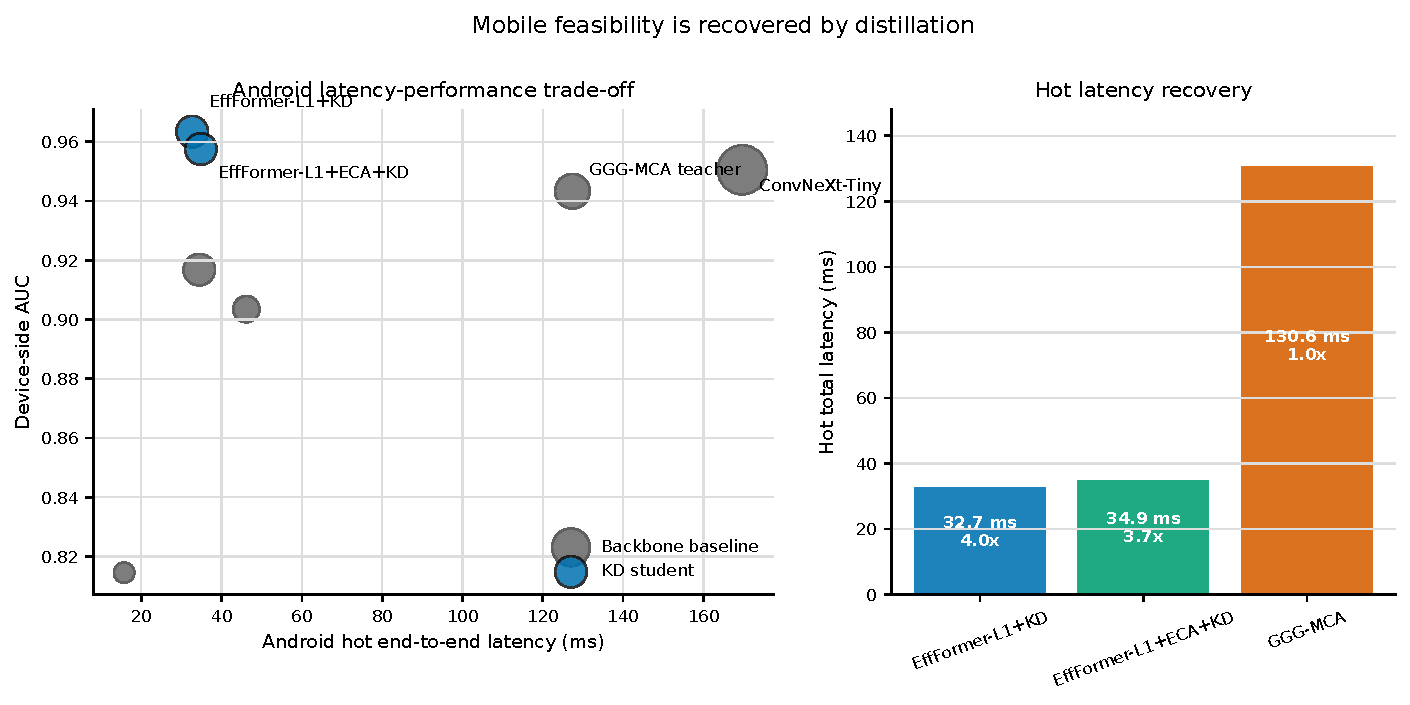
\includegraphics[width=0.92\textwidth]{fig_mobile_latency_tradeoff_crop.pdf}
    \caption{Android latency--accuracy trade-off on the Xiaomi device. Distilled EfficientFormer students occupy a more practical real-device latency region than the TransXNet-family teacher; Table~\ref{tab:mobile} reports the second-device Samsung repeat.}
    \label{fig:mobile}
\end{figure}

\subsection{Multi-organ joint training and transfer boundary}

Table~\ref{tab:cross_organ} separates three claims. Single-domain training gives per-dataset controls. Joint multi-organ training trains one shared EfficientFormer-L1+ECA model and evaluates each dataset under its own test protocol. LODO tests true held-out-organ transfer. Joint training remains reasonable, especially on BUSI and AUL, but LODO AUCs of 0.6127--0.7262 show that zero-shot cross-organ generalization is still weak. We therefore use the term multi-organ public benchmark evaluation, not cross-organ validation.

\begin{table}[!htbp]
    \centering
    \small
    \caption{Multi-organ joint training and zero-shot boundary probe with EfficientFormer-L1+ECA. Bracketed values are seed-averaged case-bootstrap 95\% confidence intervals.}
    \label{tab:cross_organ}
    \begin{adjustbox}{max width=\columnwidth}
    \begin{tabular}{lccc}
        \toprule
        Protocol & TN5000 AUC & BUSI AUC & AUL AUC \\
        \midrule
        Single-domain & 0.9380 [0.9222, 0.9524] & 0.8158 [0.7273, 0.8987] & 0.7358 [0.6394, 0.8293] \\
        Joint multi-organ & 0.9253 [0.9070, 0.9417] & 0.8195 [0.7264, 0.9056] & 0.7861 [0.7036, 0.8575] \\
        LODO zero-shot & 0.6127 & 0.6796 & 0.7262 \\
        \bottomrule
    \end{tabular}
    \end{adjustbox}
\end{table}

\begin{figure}[!htbp]
    \centering
    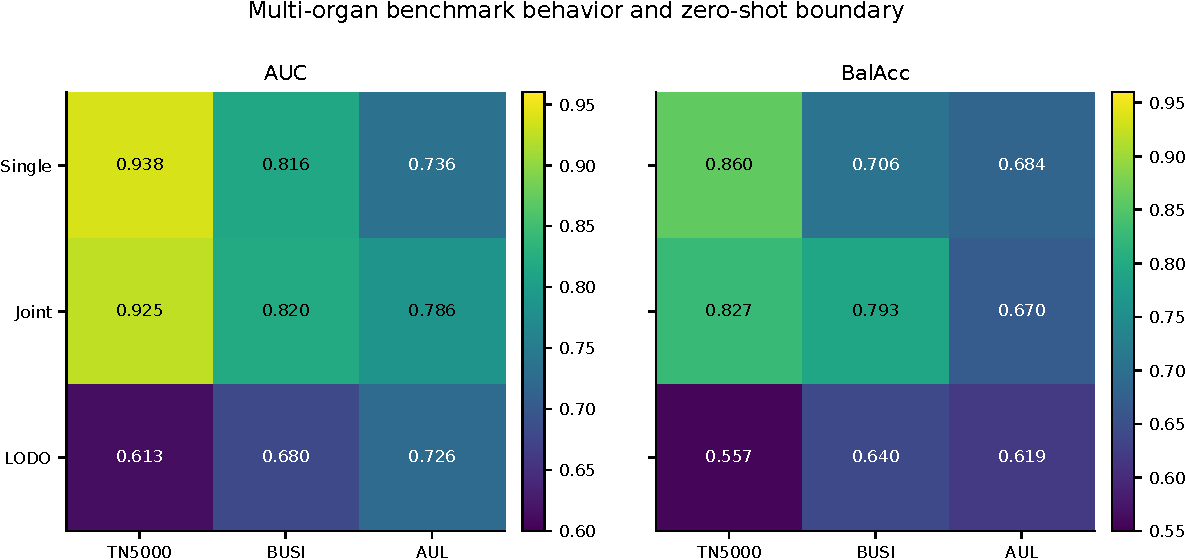
\includegraphics[width=0.92\textwidth]{fig_multi_organ_protocol_heatmap_crop.pdf}
    \caption{Protocol-separated multi-organ results. Joint training is feasible under dataset-specific testing, but leave-one-domain-out transfer remains limited.}
    \label{fig:cross_organ}
\end{figure}

\section{Discussion}
\label{sec:discussion}

The results support a more defensible story than the initial ``new backbone'' framing. High-capacity TransXNet-family models are useful for ROI classification and robustness analysis, but the most deployable model is a distilled EfficientFormer student. Likewise, multi-organ joint training is feasible, but zero-shot transfer across organs remains limited. These distinctions matter because medical imaging AI papers can look stronger than they are if oracle ROIs, dataset-specific training, threshold selection, and mobile latency are mixed into one broad claim.

The factorial ablation also changes the interpretation of the modules. MUDD and differential attention provide the most reliable TN5000 gain. MCA is not a universal AUC booster, even though it may still help some operating points and datasets. We therefore treat the TransXNet-family teacher as a design space, not as a single monotonic sequence where every added module improves every metric.

The ROI robustness experiment is the strongest practical evidence in the current package. Detector boxes and moderate synthetic noise preserve much of the GT-ROI performance, suggesting that the classifier can tolerate plausible localization error. The detector-quality tables also show that the localization front end is not uniformly strong across organs, with AUL lower than TN5000 and BUSI. The detector should therefore be read as an auxiliary front end rather than a new detection contribution. A clinical workflow would still require prospective acquisition, failure-mode handling, and explicit human-review logic.

The Android experiment similarly supports mobile feasibility but not clinical deployment. Measurements were made on one Xiaomi phone and one Samsung tablet, and runtime profile sweeps on the Xiaomi device showed that CPU execution was faster than NNAPI in this configuration. This is important for reproducibility: a small parameter count does not guarantee fast Android inference, and delegate choice can reverse expected rankings.

Calibration remains a separate constraint from discrimination. TN5000 is well calibrated after temperature scaling, but the supplementary calibration table shows higher ECE on BUSI and especially AUL. This means that AUL probability outputs should not be interpreted directly as calibrated clinical risk estimates under distribution shift, even when ranking metrics remain useful. In a clinical workflow, operating thresholds and probability communication would need dataset- or site-specific validation.

\subsection*{Limitations}

This study has several limitations. First, all datasets are retrospective public datasets, and the label definitions and acquisition conditions are not fully harmonized. The BUSI audit identifies exact and perceptual duplicate candidates, including label-conflict candidates, so BUSI results should be interpreted as public-benchmark comparability rather than a cleaned patient-level clinical estimate. Second, annotation-derived ROI crops remain the primary classifier protocol; detector-derived crops and box perturbations mitigate but do not eliminate this dependency. Third, BUSI and AUL are primarily dataset-specific benchmarks, not evidence of thyroid-to-breast or thyroid-to-liver external generalization. Fourth, mobile feasibility is measured on two Android devices and should be interpreted as prototype evidence until broader chipsets, delegates, and thermal states are measured. Fifth, model calibration remains less stable outside TN5000, especially for smaller datasets. Sixth, the label snapshot used for the added robustness and deployment analyses must be audited through released manifests and prediction CSV files, because aggregate class counts alone are not sufficient provenance. Seventh, the module innovations are adaptations and reorganizations of existing ideas; the contribution is the systematic ROI-ultrasound evaluation, robustness analysis, and deployment-oriented teacher-student path.

\section{Conclusions}
\label{sec:conclusion}

We presented an ROI-robust ultrasound lesion-classification framework that combines TransXNet-family teacher analysis, localization-error robustness evaluation, EfficientFormer student distillation, Android measurement, and multi-organ protocol separation. The main result is a bounded computing workflow: a high-capacity teacher identifies robust ROI configurations, detector and moderate box errors degrade performance gradually, and a distilled EfficientFormer student preserves high TN5000 discrimination at substantially lower real-device latency. True zero-shot cross-organ transfer remains unresolved and should be treated as future work rather than a completed claim.

\section*{CRediT authorship contribution statement}
Zihan Li: Conceptualization, Methodology, Software, Validation, Formal analysis, Investigation, Data curation, Visualization, Writing -- original draft. \\
Cong Yang: Conceptualization, Supervision, Resources, Project administration, Writing -- review and editing.

\section*{Ethics statement}
This study is a secondary computational analysis of publicly available, de-identified ultrasound datasets. No new patient data were collected by the authors. Ethical approval and informed-consent procedures are governed by the original dataset publications or data providers; therefore, no additional institutional review board approval was required for this retrospective computational study.

\section*{Declaration of generative AI and AI-assisted technologies}
During manuscript preparation, the authors used AI-assisted tools to support language editing, organization of revision evidence, and consistency checks under human oversight. The authors reviewed and edited all content and take full responsibility for the final manuscript.

\section*{Funding}
This research did not receive any specific grant from funding agencies in the public, commercial, or not-for-profit sectors.

\section*{Declaration of competing interest}
The authors declare that they have no known competing financial interests or personal relationships that could have appeared to influence the work reported in this paper.

\section*{Data availability}
The datasets analyzed in this study are publicly available from their original sources, which are cited in the manuscript. A reproducibility package is prepared for release and includes source code, file-level split/protocol manifests with hashes, original and analysis labels, ROI box coordinates where available, exclusion flags, environment specifications, table-generation scripts, Android export scripts, validation thresholds, temperature-scaling values, and prediction CSV files required for table regeneration where data licenses permit. Dataset image files, generated ROI folders, trained checkpoints, detector weights, ONNX binaries, Android packages, and full raw logs are not redistributed in the repository; they may be made available from the corresponding author upon reasonable request where permitted by dataset and software terms.

\bibliographystyle{elsarticle-num}
\bibliography{refs}

\end{document}
